% Created 2014-11-24 Mon 16:42
\documentclass[presentation]{beamer}
\usepackage[utf8]{inputenc}
\usepackage[T1]{fontenc}
\usepackage{fixltx2e}
\usepackage{graphicx}
\usepackage{longtable}
\usepackage{float}
\usepackage{wrapfig}
\usepackage{rotating}
\usepackage[normalem]{ulem}
\usepackage{amsmath}
\usepackage{textcomp}
\usepackage{marvosym}
\usepackage{wasysym}
\usepackage{amssymb}
\usepackage{hyperref}
\tolerance=1000
\usepackage{minted}
\usepackage{color}
\usepackage{listings}
\usepackage{minted}
\usepackage{xcolor}
\usemintedstyle{emacs}
\mode<beamer>{\usetheme{Madrid}}
\usetheme{default}
\author{Alexander Jueterbock}
\date{Nov 2014}
\title{Guppy ddRAD data analysis overview}
\hypersetup{
  pdfkeywords={},
  pdfsubject={},
  pdfcreator={Emacs 24.3.1 (Org mode 8.2.4)}}
\begin{document}

\maketitle



\begin{frame}[label=sec-1]{Evolve and Resequence (E\&R) studies}
\begin{figure}[htb]
\centering
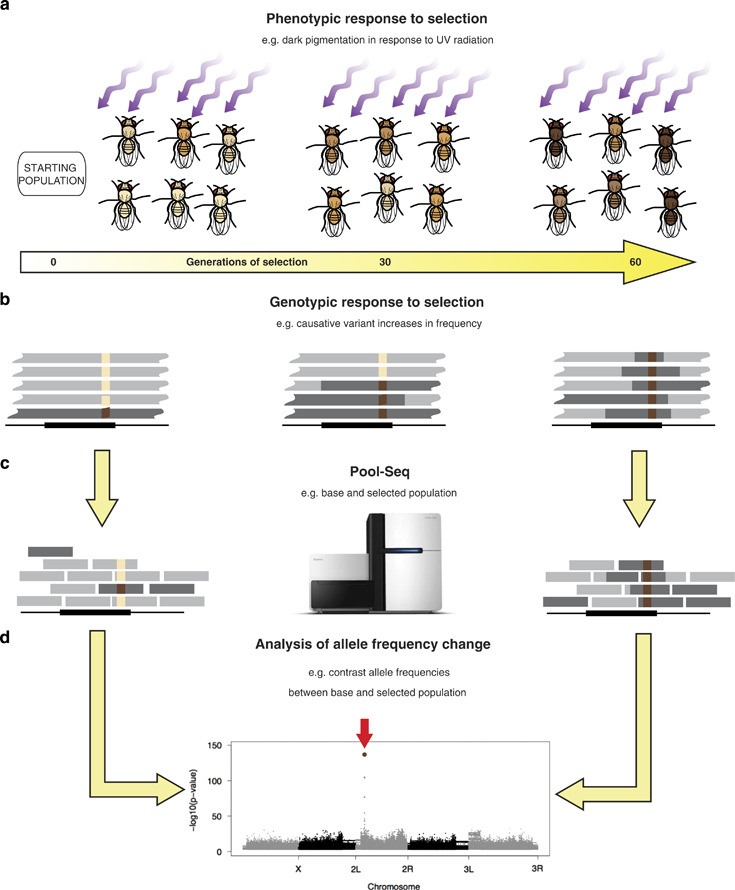
\includegraphics[width=6cm]{ERStudies.jpg}
\end{figure}
Review in Schlotterer et al. (2014)  Heredity
\end{frame}

\begin{frame}[label=sec-2]{Experiment overivew}
\begin{figure}[htb]
\centering
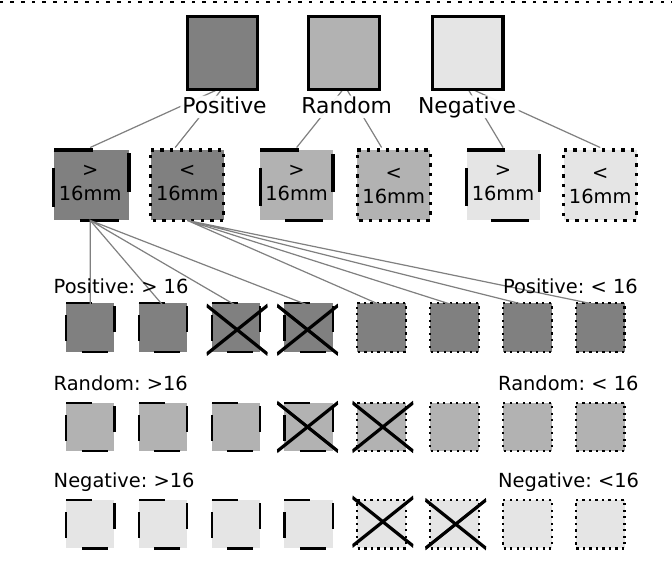
\includegraphics[width=8cm]{ExperimentalOverview.png}
\end{figure}
\end{frame}
\begin{frame}[label=sec-3]{Pooling}
\begin{itemize}
\item Critical: equimolar concentrations of individuals expected
\item Best to pool individuals at the very latest step
\item Recommended: >40 individuals/pool
\begin{itemize}
\item Higher numbers decrease 
\begin{itemize}
\item sampling error
\item unequal representation of individuals in the pool
\end{itemize}
\item But more difficult to discriminate minor allele
frequencies from sequencing errors
\end{itemize}
\end{itemize}
\end{frame}

\begin{frame}[fragile,label=sec-4]{Fastq output}
 One example sequence

(Quality scores are ASCII encoded)

\begin{minted}[]{sh}
@SEQ_ID
GATTTGGGGTTCAAAGCAGTATCGATCAAATAGTAAATCCATTTGTTCAACTC
+
!''*((((***+))%%%++)(%%%%).1***-+*''))**55CCF>>>>>>CC
\end{minted}
\end{frame}


\begin{frame}[label=sec-5]{Phred quality scores in Fastq}
\begin{figure}[htb]
\centering
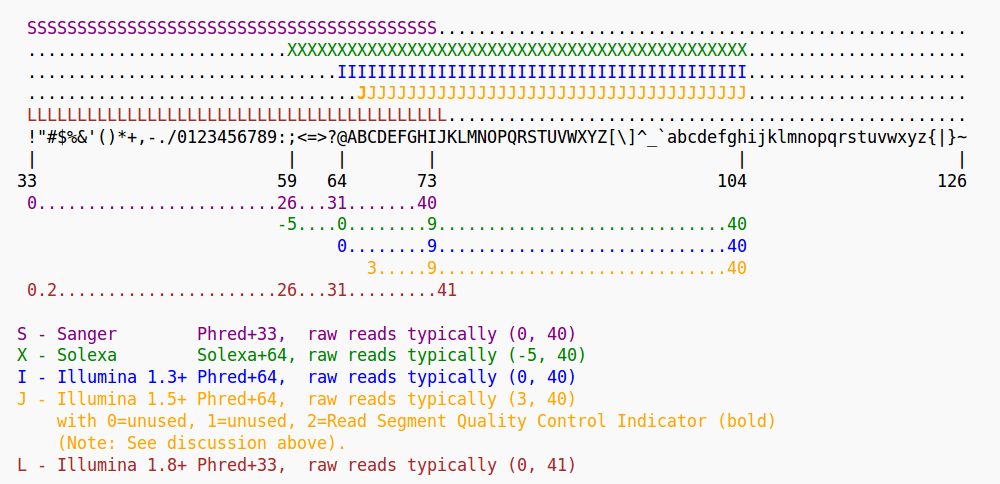
\includegraphics[width=11cm]{Fastq.png}
\caption{Quality overview of raw reads}
\end{figure}
\end{frame}


\begin{frame}[label=sec-6]{Quick and dirty analysis}
\begin{itemize}
\item DDocent Pipeline (not for pooled and replicted data)
\item STACKS (not tried, not targeted for pooled and replicated data)
\end{itemize}
\end{frame}

\begin{frame}[label=sec-7]{Demultiplexing by \textcolor{blue}{barcode}}
\begin{itemize}
\item 'process radtags' from STACKS did not work well on our data
\item DDemux used
\item Unpaired reads are discarded
\item \textcolor{blue}{Barcodes} are removed
\end{itemize}


\begin{latex:}
\footnotesize
Paired read:\\
\begin{center}
ADAPTER1 \textcolor{blue}{AATTA}\textcolor{red}{AATTC}\textcolor{green}{NNNN}CCG ADAPTER2\\
ADAPTER1 \textcolor{blue}{TTAAT}TTAAG\textcolor{green}{NNNN}\textcolor{red}{GGC} ADAPTER2
\end{center}\\
First read: \hphantom{A} \textcolor{red}{AATTC}\textcolor{green}{NNN}\\
Second read: \textcolor{red}{CGG}\textcolor{green}{NNN}\\
\vspace{0.5cm}
\textcolor{blue}{Barcode}\\
\textcolor{red}{Restriction enzyme overhang (EcoRI and MspI)}\\
\textcolor{green}{Target sequence}\\
\end{latex:}
\end{frame}

\begin{frame}[label=sec-8]{Trimming 1}
\begin{itemize}
\item I use TrimGalore!
\begin{itemize}
\item Uses 'cutadapt' for adapter trimming
\item Can handle paired end reads
\item removes orphan reads (reads without a pair)
\end{itemize}
\item Removing internal adapters (0.1\%-0.2\% of reads)
\begin{itemize}
\item Can have deviating internal barcodes
\end{itemize}
\end{itemize}
\begin{latex:}
\footnotesize
Before: \textcolor{red}{AATTC}\textcolor{green}{NNADAPTER1}\textcolor{blue}{AATTA}\textcolor{red}{AATTC}NNN\\
After: \hphantom{A}\textcolor{red}{AATTC}\textcolor{green}{NN}
\end{latex:}
\begin{itemize}
\item Minimum read length? 20bp default, I set 50bp (single sequence) as the lower limit, so 100bp paired end
\end{itemize}
\end{frame}
\begin{frame}[label=sec-9]{Trimming 2}
\begin{itemize}
\item Cut off the Restriction enzyme overhangs (5bp from read 1 and 3bp from read2)
\end{itemize}
\begin{latex:}
\footnotesize
First read: \hphantom{A} \textcolor{red}{AATTC} \textcolor{green}{NNN}\\
Second read: \textcolor{red}{CGG} \textcolor{green}{NNN}
\end{latex:}
\begin{itemize}
\item Trim bases with a Phred quality score <20 (99\% base call accurracy, Phred+33 encoding)
\end{itemize}
\begin{center}
\begin{tabular}{rll}
Phred Score & Probability of incorrect base & Base call accuracy\\
\hline
10 & 1 in 10 & 90\%\\
20 & 1 in 100 & 99\%\\
30 & 1 in 1000 & 99.9\%\\
\end{tabular}
\end{center}
\end{frame}

\begin{frame}[label=sec-10]{Read qualities before trimming}
\begin{figure}[htb]
\centering
\includegraphics[width=10cm]{FastQC/Pop1_1.fq_fastqc/Images/per_base_quality.png}
\caption{Quality before trimming}
\end{figure}
\end{frame}
\begin{frame}[label=sec-11]{Read qualities after trimming}
\begin{figure}[htb]
\centering
\includegraphics[width=10cm]{TrimmedFastQC/Pop1_1_val_1.fq_fastqc/Images/per_base_quality.png}
\caption{Quality after trimming}
\end{figure}
\end{frame}




\begin{frame}[label=sec-12]{Number of Sequences}
\begin{figure}[htb]
\centering
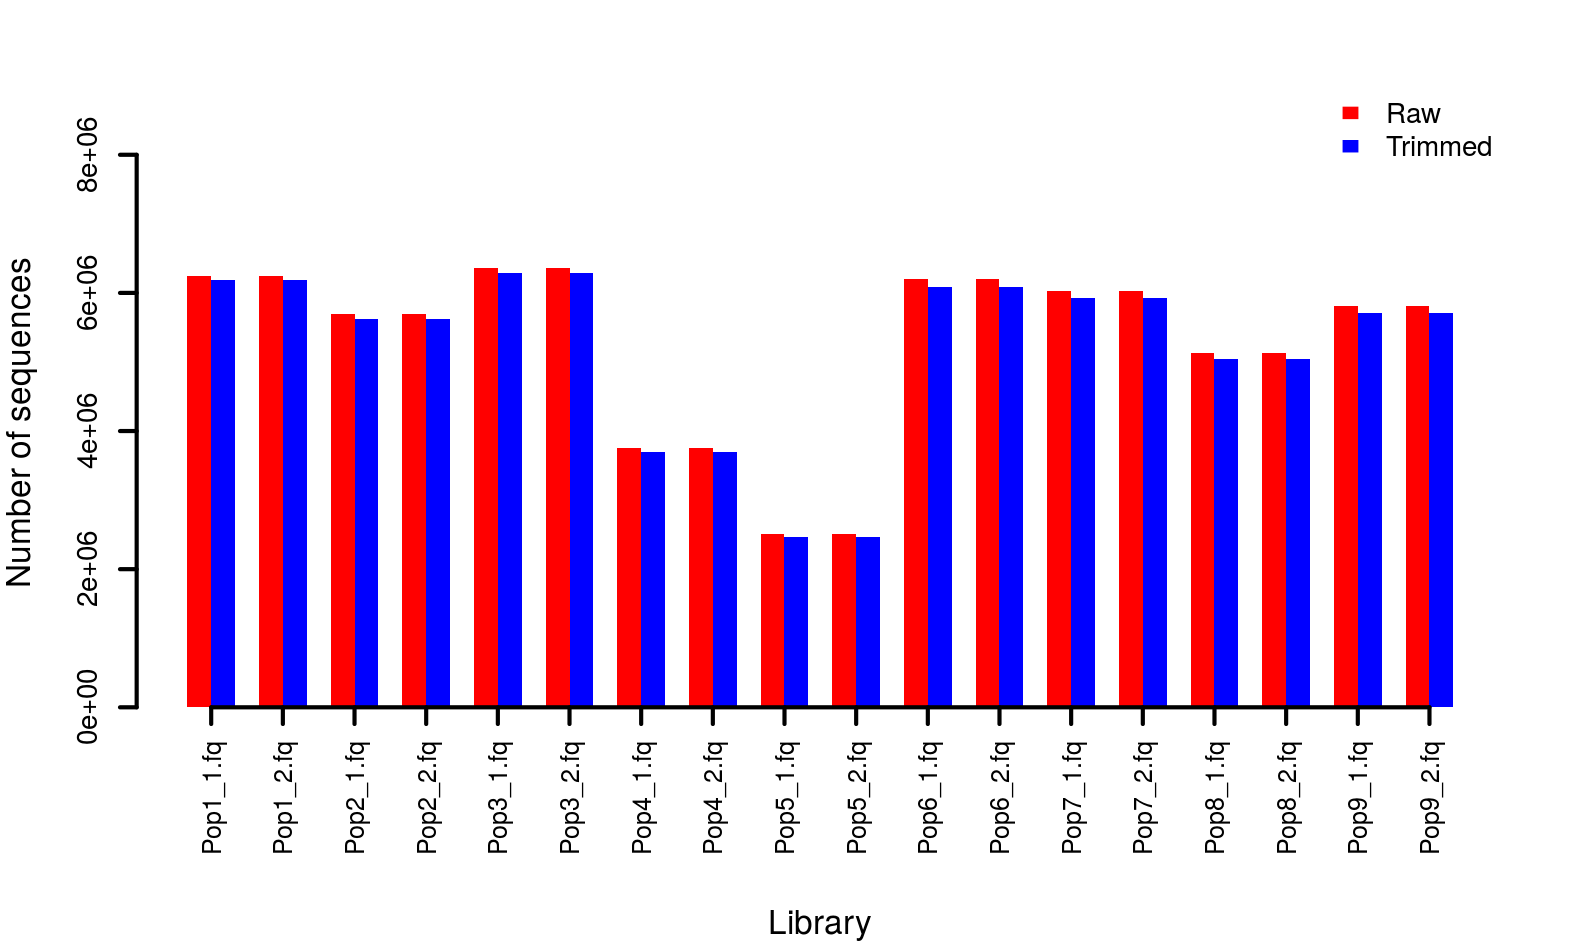
\includegraphics[width=10cm]{20141124NumberOfSequences.png}
\caption{Number of sequences}
\end{figure}
\end{frame}

\begin{frame}[label=sec-13]{CG Percentage}
\begin{figure}[htb]
\centering
\includegraphics[width=10cm]{20141124PercentageGC.png}
\caption{Percentage of GC}
\end{figure}
\end{frame}

\begin{frame}[label=sec-14]{Quality of raw reads}
\begin{figure}[htb]
\centering
\includegraphics[width=7cm]{20141124RawReads_QualityOverview.png}
\caption{Quality overview of raw reads}
\end{figure}
\end{frame}

\begin{frame}[label=sec-15]{Quality of trimmed reads}
\begin{figure}[htb]
\centering
\includegraphics[width=7cm]{20141124TrimmedReads_QualityOverview.png}
\caption{Quality overview of trimmed reads}
\end{figure}
\end{frame}
\begin{frame}[label=sec-16]{Kmer content - overrepresented sequences at the beginning}
\begin{center}
\begin{tabular}{lrr}
Sequence & Count & Obs/Exp Max\\
\hline
CCCTAGC & 5615 & 195.27312\\
CTAGCCC & 5660 & 193.232\\
GCGTTGG & 6795 & 180.89699\\
CCTAGCC & 6130 & 178.19095\\
\end{tabular}
\end{center}

\begin{itemize}
\item Overrepresented sequences due to ddRAD stacks (high duplication
levels)
\end{itemize}
\end{frame}

\begin{frame}[label=sec-17]{Duplication Percentage}
\begin{figure}[htb]
\centering
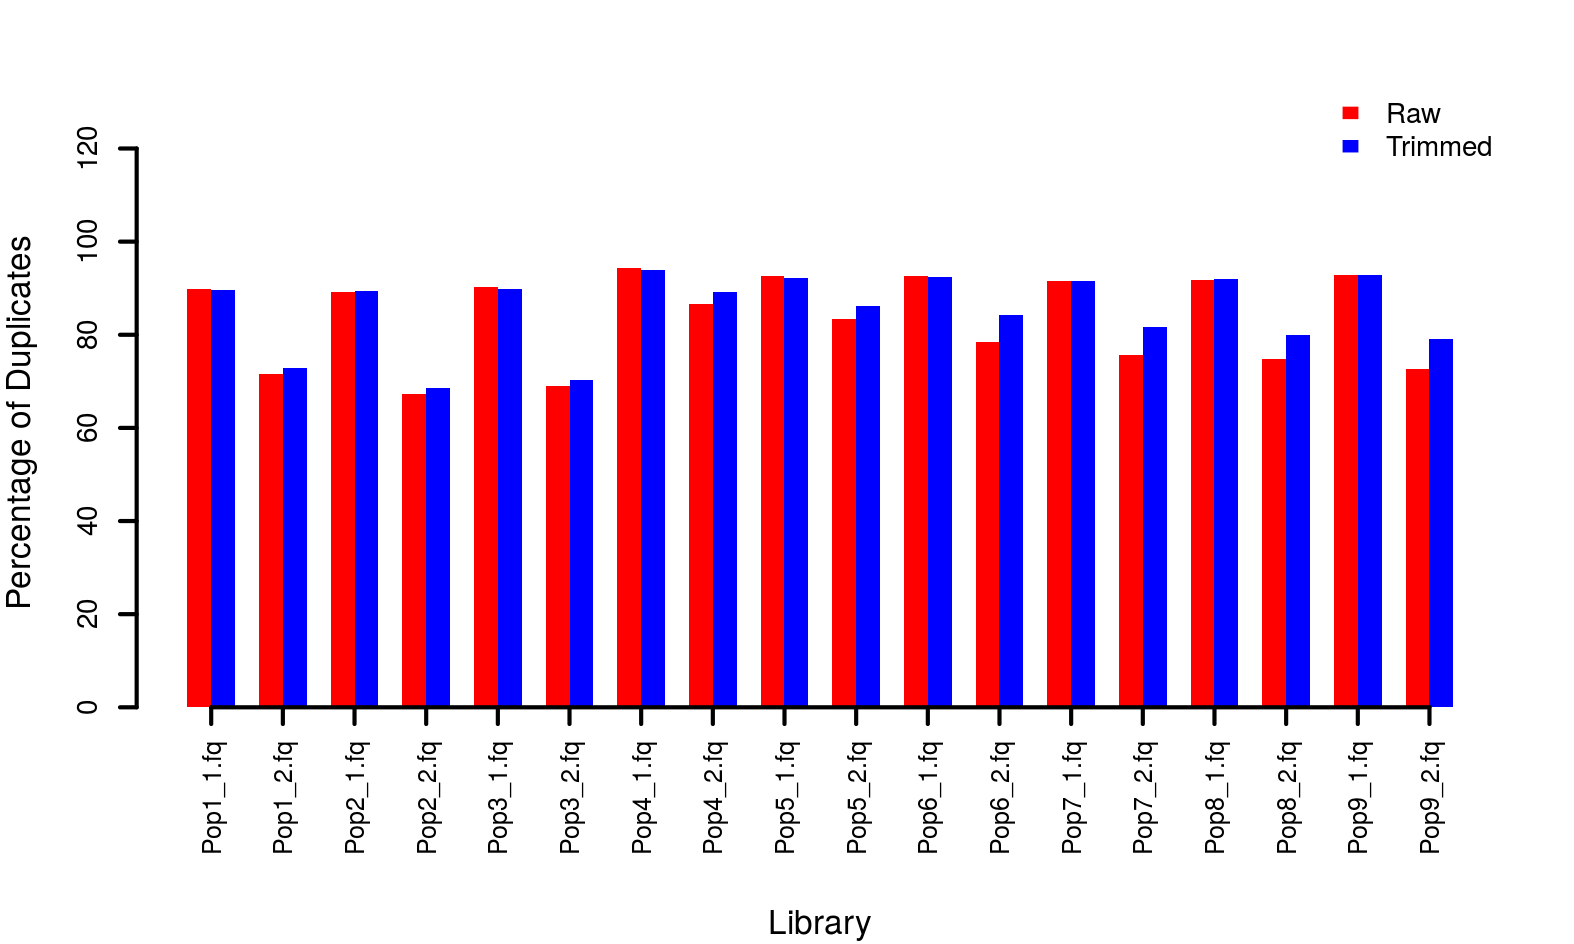
\includegraphics[width=10cm]{20141124PercentageDuplicates.png}
\caption{Percentage of Duplicates}
\end{figure}
\end{frame}
\begin{frame}[label=sec-18]{Duplication levels}
\begin{figure}[htb]
\centering
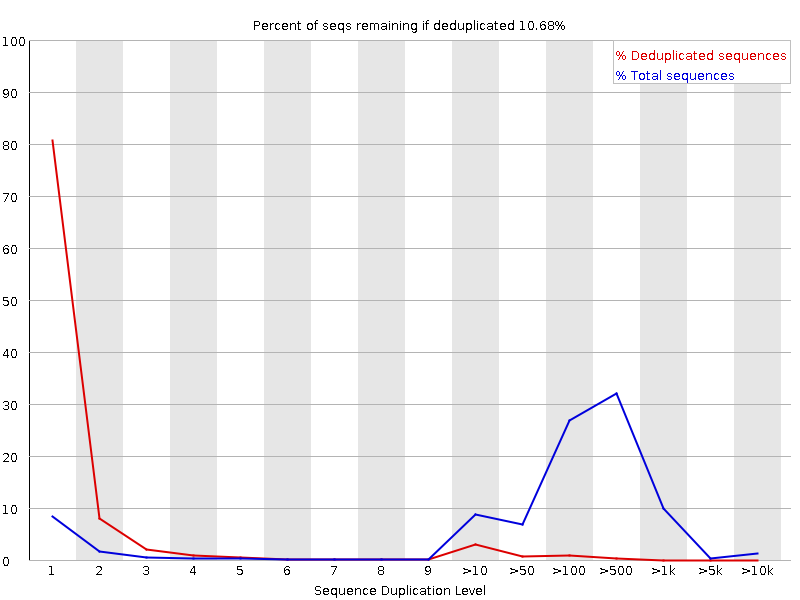
\includegraphics[width=10cm]{TrimmedFastQC/Pop1_1_val_1.fq_fastqc/Images/duplication_levels.png}
\caption{Duplication levels}
\end{figure}
\end{frame}

\begin{frame}[label=sec-19]{PCR duplicates and ddRADs can not be discriminated}
\begin{itemize}
\item RAD: equal only at one end
\item ddRAD: equal at both ends, makes identification of PCR duplicates
impossible
\item \citep{Tin2014} introduces four random bp to allow for duplicate
detection in ddRAD reads
\end{itemize}
\end{frame}

\begin{frame}[label=sec-20]{Mapping (Present state)}
\begin{itemize}
\item Recommended: 
\begin{itemize}
\item Avoid as it can cause allele frequency biases:
\begin{itemize}
\item Seeding (mapping of read subsets); reason: it discriminates
against diverged reads?!
\item Local alignment and soft-clipping (removing of terminal
mismatches)
\end{itemize}
\end{itemize}
\item Allow gaps as ungapped alignment leads to false positive SNPs and mapping inaccuracy
\item Map only proper pairs, discard broken pairs
\item I use Bowtie2 (one of the recommendations in \citep{Schlotterer2014})
\begin{itemize}
\item Uses semi-global but multi-seed alignment
\item Alternative1: BWA aln and sampe but only optimal for up to 100bp
reads
\item Alternative 2: BWA mem (used in the DDocent pipeline, but uses
seeding and local alignment)
\end{itemize}
\end{itemize}
\end{frame}

\begin{frame}[label=sec-21]{Realign around Indels}
\begin{itemize}
\item reads around indels: generally misaligned, results in false SNPS
\item istead of realigning: ignore regions around indels
\item Programs Dindel or GATK
\end{itemize}
\end{frame}

\begin{frame}[label=sec-22]{Filtering}
\begin{itemize}
\item Filter out broken pairs
\item Filter out ambiguously mapped reads? \citep{Schlotterer2014} sees
mapping quality as more important than targeting only unqiuely
mapped reads.
\item Mapping quality above 20
\end{itemize}
\end{frame}

\begin{frame}[label=sec-23]{Coverage}
\begin{itemize}
\item 50 recommended
\item 20 as the absolute minimum. What do we aim for?
\item less than 50: Sliding window analysis recommended. Only possible for species
with genome or transcriptome reference
\item Upper limit (too high coverage could result from copy number variations)
\begin{itemize}
\item twice the mean coverage
\item remove top 2\% coverages
\item mean coverage plus two standard deviations
\end{itemize}
\item Coverage heterogeneity has to be taken into account in subsequent
analyses. Or subsample to a homogenous coverage over the entire
genome.
\end{itemize}
\end{frame}
\begin{frame}[label=sec-24]{Variant detection 1}
\begin{itemize}
\item \alert{Major problem}: discriminate raw variants from sequencing errors
\begin{itemize}
\item Some set threshold for minimum allele count
\item Some remove all multiallelic SNPS \citep{Beissinger2014}
\item Inappropriate for pooled data \citep{Raineri2012}
\end{itemize}
\item Use algorithm that takes strand bias into account (only accept SNPs
that are occurring at similar frequencies on both strands)
\end{itemize}
\end{frame}
\begin{frame}[label=sec-25]{Variant detection 2}
\begin{itemize}
\item \alert{Consensus approach} (need to check in how far they are taking
coverage variation into account):
\begin{itemize}
\item Pool-hmm (corrects for site coverage variation)
\item SNVER (takes strand bias into account)
\item CRISP (takes strand bias into accunt)
\item snape (takes strand bias into accunt)
\item samtools mpileup followed by popoolation (gives a p-value for
strand bias)
\end{itemize}
\item \alert{Biological replicates (3)}:
\begin{itemize}
\item Take only SNPs that are identified in all three replicates \citep{Robasky2013}
\end{itemize}
\end{itemize}
\end{frame}

\begin{frame}[label=sec-26]{Nucleotide diversity}
\begin{itemize}
\item popoolation allows calculation of Tajima's D and Watterson's theta
\item Using a sliding window approach (window size between 5 and 50 kbp)
\end{itemize}
\end{frame}

\begin{frame}[label=sec-27]{How Tajima's D, Watterson's theta and Fst were used in our cod paper}
\begin{figure}[htb]
\centering
\includegraphics[width=10cm]{BardPaper.png}
\caption{Population genetic parameters of cod populations}
\end{figure}
\end{frame}

\begin{frame}[label=sec-28]{Adaptive differentiation}
\begin{itemize}
\item Consensus approach
\begin{itemize}
\item popoolation2 (Fisher's exact test and CMH (Cochran-Mantel-Haenzel)
test (takes biological replicates into account, used also by \citep{Huang2014})
\item pool-hmm (detection of selective sweeps)
\item Bayenv (calculates environmental correlation, so this might not be the right approach for E\&R studies)
\item SelEstim (detects and quantifies selection)
\end{itemize}

\item \alert{Replicates}: 
\begin{itemize}
\item In the CMH test taken into account
\item Do several pairwise comparison and identify overlapping outliers
\item Pool the allele frequencies before applying the test
\item Calculate a composite p-value or log-likelihood from the single tests
\end{itemize}
\end{itemize}


\begin{itemize}
\item Do we compare the selected with the non-selected populations or also
the selected with each other?
\end{itemize}
\end{frame}
\begin{frame}[label=sec-29]{Expected results}
\begin{figure}[htb]
\centering
\includegraphics[width=12cm]{CMHTestresult.png}
\caption{Manhatten plot with p-values from CMH test}
\end{figure}
\end{frame}

\begin{frame}[label=sec-30]{Annotation}
\begin{itemize}
\item Have to see what annotation of the genome is already available
\item Programs for SNP annotation: SNPeff or AnnoVar
\end{itemize}
\end{frame}
% Emacs 24.3.1 (Org mode 8.2.4)
\end{document}